% ARPEGOS:  Automatized Roleplaying-game Profile Extensible Generator Ontology based System %
% Author : Alejandro Muñoz Del Álamo %
% Copyright 2019 %

% Section 7.1: Entorno de Pruebas %
\section{Organización del código fuente}
Como se ha comentado en capítulos anteriores, el proyecto se ha desarrollado en \textit{Visual Studio}, y se ha aplicado el 
patrón de arquitectura \textit{MVVM}. \medskip

Al haber utilizado \textit{Visual Studio}, la aplicación se ha desarrollado en una \textbf{\textit{solución}}, que es un contenedor que contiene 
uno o más proyectos relacionados, junto a información de compilación, la configuración de \textit{Visual Studio} y archivos no asociados 
a un proyecto determinado. Por otro lado, un \textbf{\textit{proyecto}} es el conjunto de ficheros que se compilan en un archivo ejecutable, 
biblioteca o sitio web. \medskip

En lo referente a la solución diseñada, llamada {\textit{ARPEGOS}, disponemos de tres proyectos generales: \textit{ARPEGOS}, 
\textit{ARPEGOS\_Android} y \textit{ARPEGOS\_Unit\_Test}, tal y como se muestra en la figura\ref*{SolutionProjects}. Aparece además, 
otro proyecto llamado \textit{ARPEGOS\_iOS}, que indica que se puede desarrollar la aplicación también para \textit{iOS}, ya 
que \textit{Xamarin} permite desarrollar aplicaciones multiplataforma.


\begin{figure}[H]
    \centering
    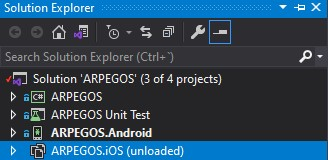
\includegraphics[scale=1.5]{Images/Solution_Projects.jpg}
    \caption{Proyectos de la solución \textit{ARPEGOS}}
    \label{SolutionProjects}    
\end{figure}

\subsection{El proyecto \textit{ARPEGOS}}
El proyecto \textit{ARPEGOS} constituye la base de la aplicación, puesto que contiene toda la lógica de negocio de la aplicación, 
independiente del dispositivo en el que se vaya a ejecutar. En la figura\ref*{SolutionARPEGOS} se muestra la estructura de este proyecto.

\begin{figure}[H]
    \centering
    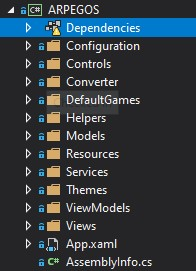
\includegraphics[scale=1.5]{Images/Solution_ARPEGOS_Project.jpg}
    \caption{Proyecto \textit{ARPEGOS}}
    \label{SolutionARPEGOS}    
\end{figure}

